\documentclass[border=3pt]{standalone}
% Preâmbulo compartilhado pelos diagramas TikZ da aula 4 de Navegação (Representação de Mapas)
\usepackage[T1]{fontenc}
\usepackage[utf8]{inputenc}
\usepackage{lmodern}
\usepackage{amsmath}
\usepackage{xcolor}
\usepackage{tikz}
\usetikzlibrary{arrows.meta,angles,quotes,decorations.pathmorphing,decorations.pathreplacing,calc,
                positioning,shapes.geometric,shapes.misc,backgrounds,fit,
                math}

% Paleta (mesma dos SVGs originais)
\definecolor{dblue}{HTML}{2A5B8C}
\definecolor{dorange}{HTML}{B3541E}
\definecolor{dgreen}{HTML}{4A7C59}
\definecolor{dred}{HTML}{9C4B4B}
\definecolor{dcream}{HTML}{F4F1EA}
\definecolor{dshade}{HTML}{DDD7C9}

% Função gaussiana (não normalizada por padrão de escala visual)
\pgfmathdeclarefunction{gauss}{3}{%
  \pgfmathparse{1/(#3*sqrt(2*pi))*exp(-((#1-#2)^2)/(2*#3^2))}%
}

% Estilos comuns (prefixo d... para não colidir com chaves internas do pgf)
\tikzset{
  >={Stealth[length=2mm]},
  dguide/.style={gray!55, dashed, line width=0.4pt},
  daxis/.style={gray!60, line width=0.7pt, ->},
  dbody/.style={fill=black!3, draw=black!80, line width=1pt},
  dacc/.style={draw=dblue, line width=1pt},
  dlbl/.style={black!55, font=\small},
  dsub/.style={black!45, font=\footnotesize},
  dstate/.style={circle, draw=black!80, fill=dcream, line width=1pt,
                 minimum size=17mm, font=\large, inner sep=1pt},
  dobs/.style={circle, draw=black!80, fill=dshade, line width=1pt,
               minimum size=14mm, font=\large, inner sep=1pt},
  dbox/.style={rounded corners=2pt, draw=black!80, fill=dcream, line width=1pt,
               align=center, inner sep=6pt},
  dop/.style={circle, draw=black!80, fill=white, line width=1pt,
              minimum size=6mm, inner sep=0pt, font=\small},
  dtrans/.style={->, dblue, line width=1pt},
  dmeas/.style={->, dorange, line width=1pt},
  dcurve/.style={line width=1pt, dblue},
  dcurveb/.style={line width=1.4pt, dorange},
}

\begin{document}
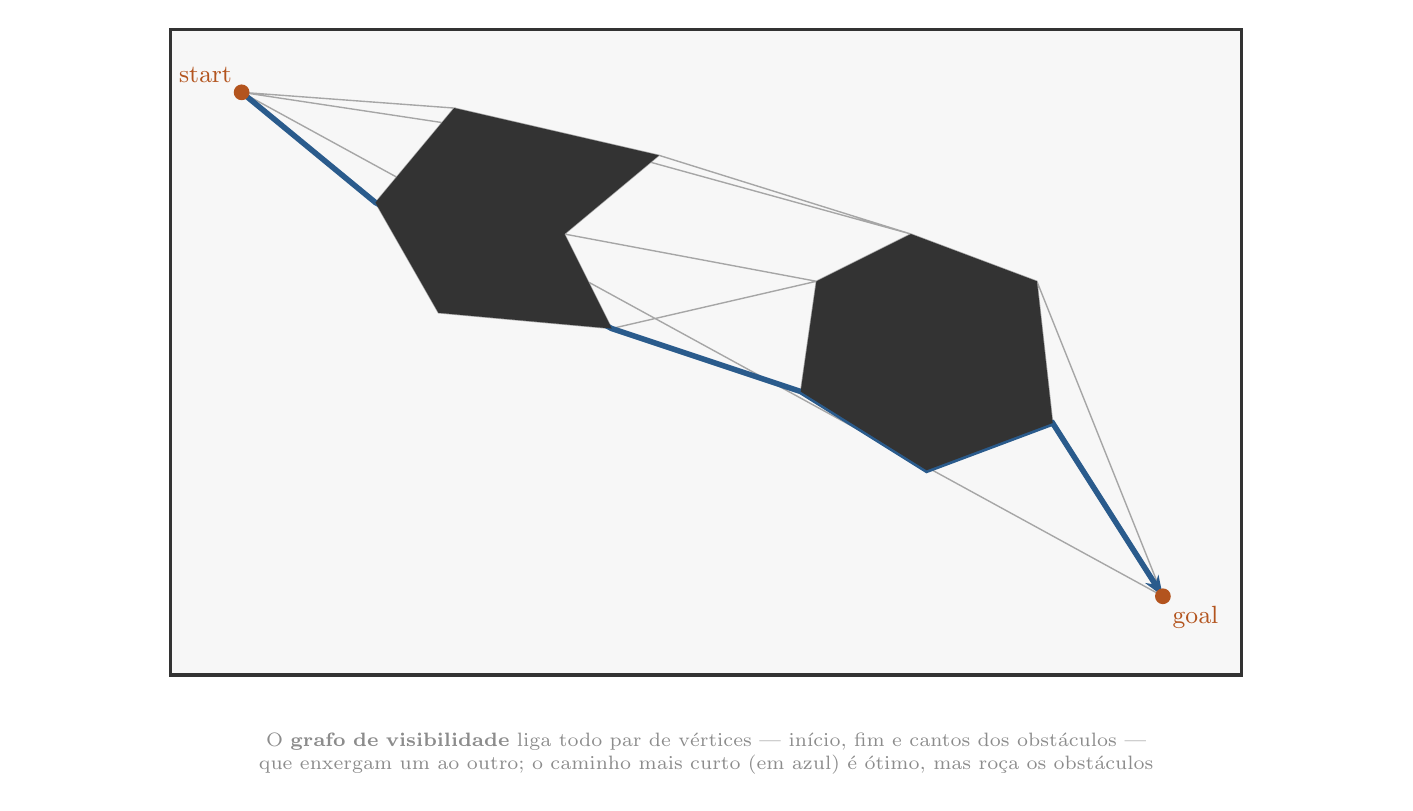
\begin{tikzpicture}[x=1cm,y=1cm]

  \draw[dbody, line width=1.2pt] (0,0) rectangle (13.6,8.2);

  \coordinate (start) at (0.9,7.4);
  \coordinate (goal) at (12.6,1.0);

  \coordinate (a1) at (3.6,7.2);
  \coordinate (a2) at (2.6,6.0);
  \coordinate (a3) at (3.4,4.6);
  \coordinate (a4) at (5.6,4.4);
  \coordinate (a5) at (5.0,5.6);
  \coordinate (a6) at (6.2,6.6);

  \coordinate (b1) at (8.0,3.6);
  \coordinate (b2) at (9.6,2.6);
  \coordinate (b3) at (11.2,3.2);
  \coordinate (b4) at (11.0,5.0);
  \coordinate (b5) at (9.4,5.6);
  \coordinate (b6) at (8.2,5.0);

  % arestas de visibilidade (finas, cinza) --- inclui os lados dos polígonos
  \draw[black!35, line width=0.5pt]
    (start) -- (a1) -- (a2) -- (a3) -- (a4) -- (a5) -- (a6) -- (a1)
    (start) -- (a2)
    (start) -- (a6)
    (a6) -- (b5)
    (a4) -- (b1)
    (a4) -- (b6)
    (a5) -- (b6)
    (b1) -- (b2) -- (b3) -- (b4) -- (b5) -- (b6) -- (b1)
    (b3) -- (goal)
    (b4) -- (goal)
    (a1) -- (b5)
    (start) -- (goal);

  % caminho mais curto (destacado)
  \draw[dblue, line width=2pt, -{Stealth[length=2.6mm]}]
    (start) -- (a2) -- (a4) -- (b1) -- (b2) -- (b3) -- (goal);

  \fill[black!80] (a1) -- (a2) -- (a3) -- (a4) -- (a5) -- (a6) -- cycle;
  \fill[black!80] (b1) -- (b2) -- (b3) -- (b4) -- (b5) -- (b6) -- cycle;

  \fill[dorange] (start) circle (0.1);
  \node[dorange, font=\small, anchor=south east] at (start) {start};
  \fill[dorange] (goal) circle (0.1);
  \node[dorange, font=\small, anchor=north west] at (goal) {goal};

  \node[dsub, font=\scriptsize, align=center, text width=17cm] at (6.8,-1.0)
     {O \textbf{grafo de visibilidade} liga todo par de vértices --- início, fim e cantos dos obstáculos --- que enxergam um ao outro; o caminho mais curto (em azul) é ótimo, mas roça os obstáculos};

\end{tikzpicture}
\end{document}
